\documentclass[convert]{standalone}

\usepackage{tikz}
\usepackage{graphicx}
\pagestyle{empty}

% INT_AY22_L28-Fig10_Faraday_law_wave.png

\begin{document}
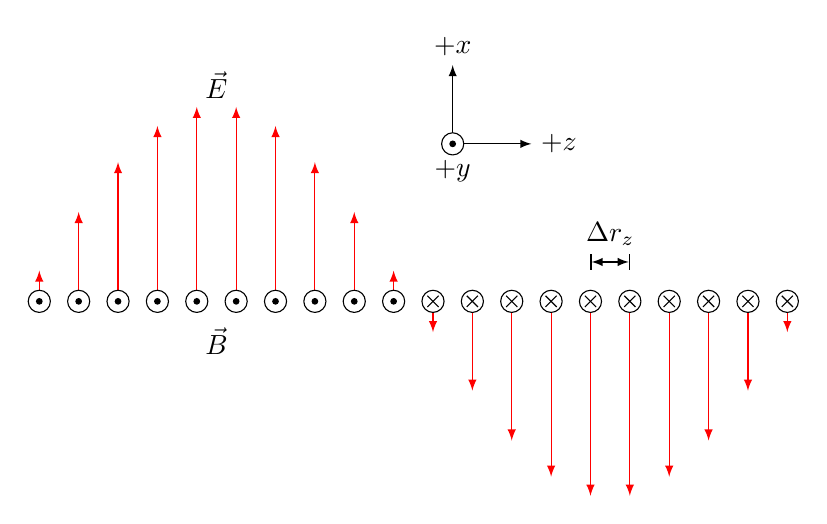
\begin{tikzpicture}[> = latex]

	% Definitions
	
	\def\E{2.5}		% Magnitude of E field
	\def\L{10}		% Wavelength
	
	% Electric field

	\foreach \x in {0.25, 0.75, ..., 10}
		\draw [red, ->] (\x, 0) -- (\x, {\E * sin(360 * \x / \L)});
		
	% Distances between points
	
	\draw [|<->|] (7.25, 0.5) -- node [above = 0.25 em] {$\Delta r_z$} (7.75, 0.5);
		
	% Magnetic field
	
	\foreach \x in {0.25, 0.75, ..., 5}
	{
		\draw [fill = white] (\x, 0) circle (4 pt);
		\filldraw (\x, 0) circle (1 pt);
	}
	
	\foreach \x in {5.25, 5.75, ..., 10}
	{
		\draw [fill = white] (\x, 0) circle (4 pt);
		\draw (\x + 0.071, 0.071) -- (\x - 0.071, -0.071);
		\draw (\x - 0.071, 0.071) -- (\x + 0.071, -0.071);
	}
	
	% Field labels
	
	\node at (2.5, 2.75) {${\vec E}$};
	\node at (2.5, -0.5) {${\vec B}$};
	
	% Coordinate axes
	
	\draw [<->] (5.5, 3) node [above] {$+x$} -- (5.5, 2) -- (6.5, 2) node [right] {$+z$};
	
	\draw [fill = white] (5.5, 2) circle (4 pt) node [below = 0.25 em] {$+y$};
	\filldraw (5.5, 2) circle (1 pt);
	
\end{tikzpicture}
\end{document}